\documentclass{article}
\usepackage{pgfplots}
\pgfplotsset{compat=1.8}


\begin{document}
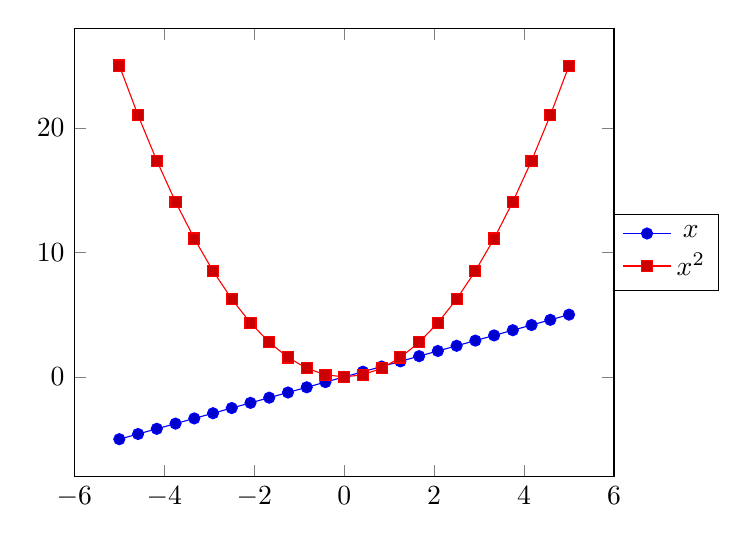
\begin{tikzpicture}
  \begin{axis}[
      legend entries={$x$,$x^2$},
      legend style={
        at={(1,0.5)},        % 1.03(>1) moves out of the graph along x, 0.5 means half-way along y
        anchor=west         %where the image will 'hang/support'. North/South/East/West means anchor will attach at ``at coordinate from top/bottom/right/left that direction. 
      }
    ]
    \addplot {x};
    \addplot {x^2};
  \end{axis}
\end{tikzpicture}

\setlength{\fboxsep}{0pt}
\fbox{
  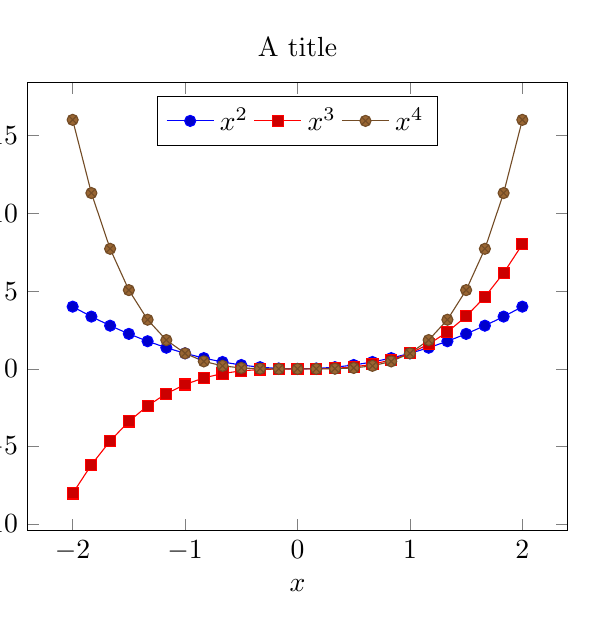
\begin{tikzpicture}
    \begin{pgfinterruptboundingbox}
      \begin{axis}[
          title=A title,
          xlabel={$x$},
          ylabel={$y$},
          legend style={at={(0.5,0.97)},
            anchor=north,legend columns=-1},
          domain=-2:2           % domain on the x axis
        ]
        \addplot {x^2};
        \addplot {x^3};
        \addplot {x^4};
        \legend{$x^2$,$x^3$,$x^4$}
      \end{axis}
    \end{pgfinterruptboundingbox}

    \useasboundingbox
    (current axis.below south west)
    rectangle (current axis.above north east);
  \end{tikzpicture}
}

\begin{tikzpicture}
  \begin{axis}[%
      scale only axis,
      width=0.45\textwidth,
      height=0.2\textheight,
      xmin=0, xmax=300,
      ymin=-2e+06, ymax=1e+07,
      legend entries={Analytic solution,GPS data,Kalman filtered},
      legend style={nodes=right},
      legend pos= south east]

    \addplot [color=blue, solid]
    coordinates{ (0,7e+06) (0.1,7.0007e+06) (0.2,7.0014e+06) };

    \addplot [color=green, solid]
    coordinates{ (0,6.99999e+06) (0.1,7.00071e+06) (0.2,7.00143e+06) };

    \addplot [color=red, solid]
    coordinates{ (0,0) (0.1,7.00071e+06) (0.2,7.00174e+06) };

  \end{axis}
\end{tikzpicture}
\end{document}
